% ============================================================================
% 格点QCD中胶子PDF计算的物理公式与GPU代码实现
% —— donghx 代码详细分析
% ============================================================================
\documentclass[12pt,a4paper]{ctexart}

% ---------- Packages ----------
\usepackage{amsmath,amssymb,amsfonts}
\usepackage{physics}
\usepackage{braket}
\usepackage{graphicx}
\usepackage{hyperref}
\usepackage{listings}
\usepackage{xcolor}
\usepackage{tcolorbox}
\usepackage{booktabs}
\usepackage{geometry}
\usepackage{fancyhdr}
\usepackage{titlesec}
\usepackage{enumitem}
\usepackage{caption}
\usepackage{subcaption}
\usepackage{fontspec}
\usepackage{tikz}
\usetikzlibrary{decorations.pathreplacing,arrows.meta,positioning,shapes}

\geometry{margin=2.5cm, headheight=14pt}
\hypersetup{
    colorlinks=true,
    linkcolor=blue,
    urlcolor=cyan,
    citecolor=green!50!black
}

% ---------- Code Style ----------
\definecolor{codebg}{RGB}{245,245,245}
\definecolor{codeframe}{RGB}{200,200,200}
\definecolor{commentgreen}{RGB}{0,128,0}
\definecolor{keywordblue}{RGB}{0,0,180}
\definecolor{stringred}{RGB}{180,0,0}

\lstdefinestyle{pythonstyle}{
    language=Python,
    backgroundcolor=\color{codebg},
    frame=single,
    rulecolor=\color{codeframe},
    basicstyle=\ttfamily\small,
    commentstyle=\color{commentgreen}\itshape,
    keywordstyle=\color{keywordblue}\bfseries,
    stringstyle=\color{stringred},
    showstringspaces=false,
    tabsize=4,
    breaklines=true,
    breakatwhitespace=false,
    numbers=left,
    numberstyle=\tiny\color{gray},
    numbersep=8pt,
    captionpos=b,
    morekeywords={contract,einsum,cp,asarray,fromfile,save,load},
}

\lstdefinestyle{bashstyle}{
    language=bash,
    backgroundcolor=\color{codebg},
    frame=single,
    basicstyle=\ttfamily\small,
    showstringspaces=false,
    breaklines=true,
    numbers=left,
    numberstyle=\tiny\color{gray},
}

% ---------- Theorem Boxes ----------
\newtcolorbox{physbox}[1][]{
    colback=blue!3!white,
    colframe=blue!50!black,
    fonttitle=\bfseries,
    title=#1
}

\newtcolorbox{codebox}[1][]{
    colback=green!3!white,
    colframe=green!50!black,
    fonttitle=\bfseries,
    title=#1
}

% ---------- Headers ----------
\pagestyle{fancy}
\fancyhf{}
\fancyhead[L]{\small 格点QCD胶子PDF计算 —— donghx代码分析}
\fancyhead[R]{\small IMP, CAS}
\fancyfoot[C]{\thepage}
\renewcommand{\headrulewidth}{0.5pt}

% ---------- Title ----------
\title{
    {\Huge \textbf{格点QCD中胶子PDF计算的}}\\[0.3cm]
    {\Huge \textbf{物理公式与GPU代码实现}}\\[0.5cm]
    {\Large —— donghx代码详细分析 ——}
}
\author{
    张欣\thanks{中国科学院近代物理研究所 (IMP, CAS)} \\[0.2cm]
    基于 /root/lattice-pdf/examples/donghx/ 中全部代码及\\
    /root/lattice-pdf/docs/ 中的参考文献
}
\date{\today}

\begin{document}

\maketitle

\tableofcontents
\newpage

% ============================================================================
% SECTION 1: 引言与物理背景
% ============================================================================
\section{引言与物理背景}

\subsection{LaMET理论框架}

大动量有效理论 (Large Momentum Effective Theory, LaMET) 是连接格点QCD欧几里得关联函数与光锥PDF的桥梁~\cite{Ji:2013dva,Ji:2014gla,Ji:2020ect}。
其核心思想是：在格点上计算一个大动量$P_z$下的准PDF (quasi-PDF) $\tilde{g}(x,P_z)$，
然后通过微扰匹配核 (perturbative matching kernel) 将其与光锥PDF $g(x,\mu)$ 联系起来：

\begin{physbox}[LaMET因子化公式]
\begin{equation}
    \tilde{g}(x, P_z) = \int_{0}^{1} \frac{dy}{|y|} \, C\pqty{\frac{x}{y}, \frac{\mu}{P_z}} \, g(y, \mu) + \mathcal{O}\pqty{\frac{\Lambda_{\text{QCD}}^2}{P_z^2}, \frac{\Lambda_{\text{QCD}}^2}{x^2 P_z^2}}
    \label{eq:lamet}
\end{equation}
\end{physbox}

其中$C(x/y, \mu/P_z)$是微扰匹配核，在NLO精度下已知。
准PDF $\tilde{g}(x,P_z)$由格点上的非定域关联函数通过Fourier变换得到：

\begin{physbox}[准PDF的Fourier变换定义]
\begin{equation}
    \tilde{g}(x, P_z) = \int_{-\infty}^{\infty} \frac{dz}{2\pi} \, e^{ixP_z z} \, \tilde{h}(z, P_z)
    \label{eq:quasi_pdf}
\end{equation}
\end{physbox}

其中$\tilde{h}(z, P_z)$是坐标空间中的非定域关联函数（IOG关联函数），
对于胶子PDF，它由场强张量$F_{\mu\nu}$构造。

\subsection{胶子PDF的矩阵元}

对于质子中的非极化胶子PDF，我们要计算的矩阵元是~\cite{Note_of_gluon_PDFs,First_Nucleon_Gluon_PDF}：

\begin{physbox}[胶子PDF矩阵元 — 内部note Eq(20)]
\begin{equation}
    \tilde{h}(z, P_z) = \frac{\braket{P | \mathcal{O}_{\mu\nu;\rho\sigma}(z) | P}}{\braket{P|P}}
    \label{eq:matrix_element}
\end{equation}

其中非定域胶子算符为：
\begin{equation}
    \mathcal{O}_{\mu\nu;\rho\sigma}(z) = F_{\mu\nu}(0) \, U(0 \to z\hat{n}) \, F_{\rho\sigma}(z\hat{n}) \, U(z\hat{n} \to 0)
    \label{eq:gluon_operator}
\end{equation}
\end{physbox}

这里$F_{\mu\nu}$是胶子场强张量，$U(0\to z\hat{n})$是沿方向$\hat{n}$的Wilson线（规范连接）。
在非极化情况下，我们需要对Lorentz指标$(\mu\nu)$和$(\rho\sigma)$求和。
在格点上，$F_{\mu\nu}$由四叶草(Clover) plaquette构造，
Wilson线由规范链路上的SU(3)矩阵乘积给出。

\subsection{非连通图与OPE分解}

胶子PDF涉及非连通图(disconnected diagram)。三点关联函数可以分解为质子2pt关联函数与OPE（Operator Product Expansion）部分~\cite{Note_of_gluon_PDFs}：

\begin{physbox}[三点关联函数的OPE分解 — 内部note Eq(25)]
\begin{equation}
    C_3(t, \tau; \vec{P}) = \sum_{\vec{x}} e^{-i\vec{P}\cdot\vec{x}} \,
    \braket{ \chi(\vec{x}, t) \, \mathcal{O}_{\text{gluon}}(z, \tau) \, \bar{\chi}(\vec{0}, 0) }
    \approx C_2(t; \vec{P}) \cdot \mathcal{O}_{\text{OPE}}(z, \tau)
    \label{eq:three_pt_decomp}
\end{equation}
\end{physbox}

因此，整个计算分为两个独立的部分：
\begin{enumerate}[label=(\arabic*)]
    \item \textbf{质子2pt关联函数} $C_2(t; \vec{P})$：使用动量涂抹(momentum smearing)的蒸馏(distillation)方法计算
    \item \textbf{OPE胶子算符} $\mathcal{O}_{\text{OPE}}(z, \tau)$：由场强张量和Wilson线构造的非定域算符
\end{enumerate}

% ============================================================================
% SECTION 2: 规范场与数据I/O
% ============================================================================
\section{规范场读入与数据组织}

\subsection{ILDG二进制格式}

格点规范组态以ILDG (International Lattice Data Grid) 二进制格式存储。
在donghx的代码中，规范场按以下方式读取（参考 \texttt{Calc\_pla.py} 和 \texttt{Calc\_ope\_unpol.py}）：

\begin{codebox}[规范场读入 — Calc\_pla.py:29-41]
\begin{lstlisting}[style=pythonstyle]
f = open("%s" % conf_file, "rb")
gauge = np.fromfile(f, dtype=">f8")
gauge = np.array(gauge)

gauge = gauge.reshape(Nt, Nx, Nx, Nx, 4, 3, 3, 2)
gauge = gauge[..., 0] + gauge[..., 1] * 1j
f.close()
\end{lstlisting}
\end{codebox}

\begin{physbox}[规范场张量结构]
读取并reshape后，规范链路的张量形状为：
\begin{equation}
    U_\mu(x) \;\longleftrightarrow\; \texttt{gauge[t, z, y, x, dir, color\_row, color\_col]}
\end{equation}
即 \texttt{[Nt, Nz, Ny, Nx, 4, 3, 3]} 的复数张量。

\textbf{空间指标约定}（donghx代码）：
\begin{itemize}
    \item 轴0: t (时间方向), 轴1: z, 轴2: y, 轴3: x
    \item 方向 $\mu$: 0=x, 1=y, 2=z, 3=t
    \item 颜色指标 (0,1,2): SU(3) 基本表示
\end{itemize}

\textbf{注意}：这与zhangxin代码中的约定不同（后者使用 \texttt{[color, color, dir, x, y, z, t]}），
在跨代码使用时需要transpose操作。
\end{physbox}

\subsection{参数传递方式}

donghx的代码使用stdin重定向方式传递参数（而非argparse），参数格式为空格分隔的键值对：

\begin{codebox}[参数传递 — Calc\_ope\_unpol.py:20-37]
\begin{lstlisting}[style=pythonstyle]
infile = fileinput.input()
for line in infile:
    tmp = line.split()
    if tmp[0] == "Nt":
        Nt = int(tmp[1])
    if tmp[0] == "Nx":
        Nx = int(tmp[1])
    if tmp[0] == "delta_z":
        delta_z = int(tmp[1])
    if tmp[0] == "conf_id":
        conf_id = tmp[1]
    if tmp[0] == "conf_file":
        conf_file = tmp[1]
    if tmp[0] == "output_dir":
        output_dir = tmp[1]
\end{lstlisting}
\end{codebox}

运行时通过shell重定向传入参数文件：
\begin{lstlisting}[style=bashstyle]
python Calc_ope_unpol.py < params.txt
\end{lstlisting}

典型的 \texttt{params.txt} 内容：
\begin{verbatim}
Nt 64
Nx 32
delta_z 15
conf_id 20000
conf_file /path/to/config.dat
link_dir z
output_dir /path/to/output/
\end{verbatim}

% ============================================================================
% SECTION 3: 场强张量F_{μν}的格点构造
% ============================================================================
\section{场强张量 $F_{\mu\nu}$ 的格点构造}

\subsection{物理定义：从Plaquette到 $F_{\mu\nu}$}

在连续极限下，规范场强张量$F_{\mu\nu}$由Wilson loop的$1\times 1$ plaquette给出：

\begin{physbox}[Plaquette与场强张量的关系]
$1\times 1$ plaquette在点$x$处的定义为：
\begin{equation}
    P_{\mu\nu}(x) = U_\mu(x) U_\nu(x+\hat{\mu}) U_\mu^\dagger(x+\hat{\nu}) U_\nu^\dagger(x)
    \label{eq:plaquette}
\end{equation}

在连续极限$a\to 0$下：
\begin{equation}
    P_{\mu\nu}(x) = \exp\pqty{i a^2 g F_{\mu\nu}(x) + \mathcal{O}(a^3)}
    \approx \mathbb{1} + i a^2 g F_{\mu\nu}(x)
    \label{eq:plaquette_exp}
\end{equation}

因此场强张量可以从plaquette的反厄米无迹部分提取：
\begin{equation}
    F_{\mu\nu}(x) = \frac{1}{2i a^2 g} \pqty{P_{\mu\nu}(x) - P_{\mu\nu}^\dagger(x)} - \frac{1}{3}\text{Tr}[\cdots]
    \label{eq:F_from_P}
\end{equation}
\end{physbox}

\subsection{Clover（四叶草）Plaquette改进}

为提高精度，实际计算中使用clover（四叶草）改进的plaquette。
Clover构型在点$x$周围使用四个plaquette的对称组合，将离散化误差从$\mathcal{O}(a)$降低到$\mathcal{O}(a^2)$：

\begin{physbox}[Clover改进的场强张量]
\begin{equation}
    F_{\mu\nu}^{\text{clover}}(x) = -\frac{i}{8a^2g} \Big[
        Q_{\mu\nu}(x) - Q_{\mu\nu}^\dagger(x)
    \Big]_{\text{traceless}}
    \label{eq:clover_F}
\end{equation}

其中$Q_{\mu\nu}$是四个定向plaquette的和：
\begin{equation}
    Q_{\mu\nu}(x) = P_{\mu\nu}(x) + P_{\nu,-\mu}(x) + P_{-\mu,-\nu}(x) + P_{-\nu,\mu}(x)
    \label{eq:Q_clover}
\end{equation}

四个plaquette从同一点$x$出发，分别沿$(\mu,\nu)$, $(\nu,-\mu)$, $(-\mu,-\nu)$, $(-\nu,\mu)$方向：
\begin{itemize}
    \item $P_{\mu\nu}$: 右上方 $1\times 1$ plaquette
    \item $P_{\nu,-\mu}$: 左上方，从$x$沿$+\nu$再沿$-\mu$
    \item $P_{-\mu,-\nu}$: 左下方，从$x$沿$-\mu$再沿$-\nu$
    \item $P_{-\nu,\mu}$: 右下方，从$x$沿$-\nu$再沿$+\mu$
\end{itemize}
\end{physbox}

\begin{center}
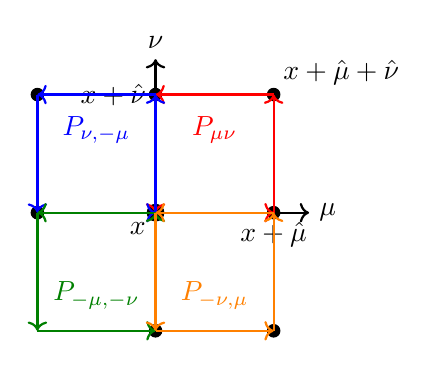
\begin{tikzpicture}[scale=1.5]
    % Central point
    \filldraw (0,0) circle (2pt) node[below left] {$x$};
    % Axes
    \draw[->,thick] (0,0) -- (1.3,0) node[right] {$\mu$};
    \draw[->,thick] (0,0) -- (0,1.3) node[above] {$\nu$};
    % Points
    \filldraw (1,0) circle (1.5pt) node[below] {$x+\hat{\mu}$};
    \filldraw (0,1) circle (1.5pt) node[left] {$x+\hat{\nu}$};
    \filldraw (1,1) circle (1.5pt) node[above right] {$x+\hat{\mu}+\hat{\nu}$};
    \filldraw (-1,0) circle (1.5pt);
    \filldraw (0,-1) circle (1.5pt);
    \filldraw (-1,1) circle (1.5pt);
    \filldraw (1,-1) circle (1.5pt);
    % P_{mu,nu} (右上)
    \draw[->,red,thick] (0,0) -- (1,0);
    \draw[->,red,thick] (1,0) -- (1,1);
    \draw[->,red,thick] (1,1) -- (0,1);
    \draw[->,red,thick] (0,1) -- (0,0);
    \node[red] at (0.5,0.7) {$P_{\mu\nu}$};
    % P_{nu,-mu} (左上)
    \draw[->,blue,thick] (0,0) -- (0,1);
    \draw[->,blue,thick] (0,1) -- (-1,1);
    \draw[->,blue,thick] (-1,1) -- (-1,0);
    \draw[->,blue,thick] (-1,0) -- (0,0);
    \node[blue] at (-0.5,0.7) {$P_{\nu,-\mu}$};
    % P_{-mu,-nu} (左下)
    \draw[->,green!50!black,thick] (0,0) -- (-1,0);
    \draw[->,green!50!black,thick] (-1,0) -- (-1,-1);
    \draw[->,green!50!black,thick] (-1,-1) -- (0,-1);
    \draw[->,green!50!black,thick] (0,-1) -- (0,0);
    \node[green!50!black] at (-0.5,-0.7) {$P_{-\mu,-\nu}$};
    % P_{-nu,mu} (右下)
    \draw[->,orange,thick] (0,0) -- (0,-1);
    \draw[->,orange,thick] (0,-1) -- (1,-1);
    \draw[->,orange,thick] (1,-1) -- (1,0);
    \draw[->,orange,thick] (1,0) -- (0,0);
    \node[orange] at (0.5,-0.7) {$P_{-\nu,\mu}$};
\end{tikzpicture}

图: Clover（四叶草）plaquette构型：从点$x$出发的四个定向plaquette
\end{center}

\subsection{代码实现：plaquette\_clover\_new}

\begin{codebox}[单个Clover Plaquette计算 — Operator.py:77-161]
\begin{lstlisting}[style=pythonstyle]
def plaquette_clover_new(gauge, mu, nu):
    # 四个起始点：通过roll操作平移整格
    gauge_rightup = gauge
    gauge_leftup = np.roll(gauge, 1, 3 - mu)
    gauge_rightdown = np.roll(gauge, 1, 3 - nu)
    gauge_leftdown = np.roll(gauge_leftup, 1, 3 - nu)

    # --- P_{mu,nu} (pla_rightup) ---
    pla_rightup = np.einsum(
        "tzyxab,tzyxbc->tzyxac",
        gauge_rightup[:, :, :, :, mu, :, :],
        np.roll(gauge_rightup, -1, 3 - mu)[:, :, :, :, nu, :, :],
    )
    pla_rightup = np.einsum(
        "tzyxab,tzyxcb->tzyxac",
        pla_rightup,
        np.roll(gauge_rightup, -1, 3 - nu)[:, :, :, :, mu, :, :].conj(),
    )
    pla_rightup = np.einsum(
        "tzyxab,tzyxcb->tzyxac",
        pla_rightup,
        gauge_rightup[:, :, :, :, nu, :, :].conj(),
    )
    # ... (类似地计算 pla_leftup, pla_leftdown, pla_rightdown)

    ans = (
        pla_rightup - pla_rightup.conj().transpose(0,1,2,3,5,4)
        + pla_leftup - pla_leftup.conj().transpose(0,1,2,3,5,4)
        + pla_leftdown - pla_leftdown.conj().transpose(0,1,2,3,5,4)
        + pla_rightdown - pla_rightdown.conj().transpose(0,1,2,3,5,4)
    )
    return -1j * ans / 8.0
\end{lstlisting}
\end{codebox}

\begin{physbox}[代码-物理对应：Clover Plaquette]
代码中的每个\texttt{einsum}对应一个SU(3)矩阵乘法（沿封闭路径的颜色指标缩并）：

\begin{itemize}
    \item \texttt{einsum("tzyxab,tzyxbc->tzyxac", A, B)}: $A_{ab} B_{bc} = (AB)_{ac}$
    \item \texttt{einsum("tzyxab,tzyxcb->tzyxac", A, B)}: $A_{ab} B_{cb} = A_{ab} (B^\dagger)_{bc} = (AB^\dagger)_{ac}$
    \item \texttt{np.roll(gauge, -1, 3-mu)}: 空间平移 $x \to x+\hat{\mu}$（将格点指标沿$\mu$方向偏移）
    \item \texttt{.conj()}: 厄米共轭 $U^\dagger$
    \item 最终返回的 \texttt{-1j * ans / 8.0}: $-\frac{i}{8} Q_{\mu\nu}^{\text{anti-hermitian}}$
\end{itemize}

四个plaquette的遍历顺序利用了$\varepsilon^{\mu\nu\rho\sigma}$的反对称性：
$P_{\mu\nu}$与$P_{\nu\mu}$给出相反的贡献，因此最终结果自然满足$F_{\mu\nu} = -F_{\nu\mu}$。
\end{physbox}

\subsection{代码实现：plaquette\_clover\_all\_new}

该函数遍历所有$(\mu,\nu)$组合生成完整的4×4 plaquette张量：

\begin{codebox}[全部plaquette生成 — Operator.py:164-174]
\begin{lstlisting}[style=pythonstyle]
def plaquette_clover_all_new(gauge, Nt, Nx):
    pla = np.zeros((4, 4, Nt, Nx, Nx, Nx, 3, 3), dtype=complex)
    Temp_zeros = np.zeros((Nt, Nx, Nx, Nx, 3, 3), dtype=complex)
    for _mu in range(4):
        for _nu in range(4):
            if _mu == _nu:
                pla[_mu, _nu] = Temp_zeros  # 对角元为0 (反对称性)
            else:
                pla[_mu, _nu] = plaquette_clover_new(gauge, _mu, _nu)
    return pla
\end{lstlisting}
\end{codebox}

输出张量形状为 \texttt{[4, 4, Nt, Nz, Ny, Nx, 3, 3]}：
\begin{itemize}
    \item 前两个维度: $(\mu,\nu)$空间方向指标
    \item 中间四个维度: 时空坐标 $(t,z,y,x)$
    \item 最后两个维度: SU(3)颜色矩阵
\end{itemize}

\subsection{对偶Plaquette：$\tilde{P}_{\mu\nu}$的构造}

胶子OPE算符中需要使用对偶场强张量 $\tilde{F}_{\mu\nu} = \frac{1}{2}\varepsilon_{\mu\nu\rho\sigma}F_{\rho\sigma}$。
代码中通过\texttt{Tensor4}（即$\frac{1}{2}\varepsilon_{\mu\nu\rho\sigma}$）将对偶变换实现为张量缩并：

\begin{codebox}[对偶Plaquette — Operator.py:177-184]
\begin{lstlisting}[style=pythonstyle]
Tensor4 = np.zeros((4, 4, 4, 4), dtype=complex)
# ... 构造 epsilon 张量: Tensor4[i,j,k,l] = 1/2 * epsilon_{i,j,k,l}
# 当(i,j,k,l)为偶排列时取 +1/2，奇排列时取 -1/2

def plaquette_clover_all_tilde(pla_all, Nt, Nx):
    pla_tilde = contract(
        "opmn,mntzyxab->optzyxab",
        Tensor4,  # (1/2) * epsilon_{mu,nu,rho,sigma}
        pla_all,  # F_{rho,sigma}(x)
    )
    return pla_tilde
\end{lstlisting}
\end{codebox}

\begin{physbox}[对偶变换的数学表达]
\begin{equation}
    \tilde{P}_{\mu\nu}(x) = \frac{1}{2} \varepsilon_{\mu\nu\rho\sigma} \, P_{\rho\sigma}(x)
    \label{eq:dual_plaquette}
\end{equation}

在胶子OPE中，非极化矩阵元需要 $F_{\mu\nu}$ 与 $\tilde{F}_{\mu\nu}$ 的组合：
\begin{equation}
    \mathcal{O}_{\text{unpol}} \sim F_{\mu\nu}(0) \, U(0\to z) \, \tilde{F}_{\mu\nu}(z) \, U(z\to 0)
\end{equation}
（注意：实际的非极化算符根据note Eq(25)有不同的Lorentz结构组合。）
\end{physbox}

% ============================================================================
% SECTION 4: 非定域胶子OPE算符
% ============================================================================
\section{非定域胶子OPE算符的构造}

\subsection{带Wilson线的非定域算符}

OPE算符的一般形式~\cite{Note_of_gluon_PDFs,Gluon_Quasi_PDF}是：

\begin{physbox}[非定域胶子算符]
\begin{equation}
    \mathcal{O}_{\mu\nu;\rho\sigma}(z\hat{n}) =
    F_{\mu\nu}(0) \,
    \underbrace{U(0\to z\hat{n})}_{\text{Wilson线}} \,
    F_{\rho\sigma}(z\hat{n}) \,
    \underbrace{U(z\hat{n}\to 0)}_{\text{返回的Wilson线}}
    \label{eq:nonlocal_op}
\end{equation}

在格点上，Wilson线是沿路径的规范链路乘积：
\begin{equation}
    U(0\to z\hat{n}) = \prod_{k=0}^{z/a-1} U_{n}(k a \hat{n})
    \label{eq:wilson_line}
\end{equation}

返回路径由厄米共轭给出：$U(z\hat{n}\to 0) = U(0\to z\hat{n})^\dagger$
\end{physbox}

\subsection{完整OPE算符的代码实现}

代码提供了多种OPE算符实现，对应不同的空间结构和边界条件。
以\texttt{operators\_new\_z0\_mu2}（最完整的带完整Wilson线的实现）为例：

\begin{codebox}[完整OPE算符 — Operator.py:339-368]
\begin{lstlisting}[style=pythonstyle]
def operators_new_z0_mu2(gauge, zdir, pla, pla_tilde,
                          delta_z, mu, nu, mu2, nu2, Nt):
    op = np.zeros(Nt, dtype=complex)
    z_dir = zdir  # Wilson线方向: 0=x, 1=y, 2=z

    # Step 1: 将F_{mu,nu}平移到位置 z-dz
    ope = np.roll(pla[mu, nu], -delta_z, 3 - z_dir)

    # Step 2: 构造返回的Wilson线 U(dz->0) = 从dz沿-z方向回来
    for _dz in range(delta_z):
        ope = np.einsum(
            "tzyxab,tzyxcb->tzyxac",
            ope,
            np.roll(gauge, -(delta_z - 1 - _dz), 3 - z_dir)[
                :, :, :, :, z_dir, :, :
            ].conj(),
        )

    # Step 3: 乘上位置0处的对偶plaquette tilde{F}_{mu2,nu2}
    ope = np.einsum(
        "tzyxab,tzyxbc->tzyxac",
        ope,
        pla_tilde[mu2, nu2],
    )

    # Step 4: 构造向前的Wilson线 U(0->dz)
    for _dz in range(delta_z):
        ope = np.einsum(
            "tzyxab,tzyxbc->tzyxac",
            ope,
            np.roll(gauge, -_dz, 3 - z_dir)[:, :, :, :, z_dir, :, :],
        )

    # Step 5: 对颜色空间取迹，对空间求和
    ans = np.trace(ope, axis1=4, axis2=5)
    op = np.sum(ans, axis=(1, 2, 3))

    return op  # shape: [Nt]
\end{lstlisting}
\end{codebox}

\begin{physbox}[代码-物理对应：OPE算符构造]
\begin{center}
\begin{tikzpicture}[scale=1.0]
    % Lattice sites
    \filldraw (0,0) circle (3pt) node[below] {$0$};
    \filldraw (3,0) circle (3pt) node[below] {$z$};
    \filldraw (6,0) circle (3pt);
    \filldraw (9,0) circle (3pt);
    \filldraw (12,0) circle (3pt) node[below] {$\delta z$};

    % Gauge links (forward Wilson line)
    \draw[->,blue,very thick] (0.3,0) -- (2.7,0);
    \draw[->,blue,very thick] (3.3,0) -- (5.7,0);
    \draw[->,blue,very thick] (6.3,0) -- (8.7,0);
    \draw[->,blue,very thick] (9.3,0) -- (11.7,0);
    \node[blue] at (6,0.4) {$U(0\to\delta z)$: 正向Wilson线};

    % Plaquette at z=0
    \draw[red,thick] (-0.5,-0.5) rectangle (0.5,0.5);
    \node[red] at (0,-1.0) {$F_{\mu\nu}(0)$};

    % Plaquette at z=dz
    \draw[red,thick] (11.5,-0.5) rectangle (12.5,0.5);
    \node[red] at (12,-1.0) {$\tilde{F}_{\mu_2\nu_2}(\delta z)$};

    % Return Wilson line
    \draw[->,green!50!black,very thick,dashed] (11.7,0.3) to[bend left=30] (0.3,0.3);
    \node[green!50!black] at (6,1.0) {$U^\dagger$: 返回Wilson线};

    % Bracket
    \draw[decorate,decoration={brace,mirror,amplitude=10pt}] (-0.8,-1.3) -- (12.8,-1.3)
        node[midway,below=12pt] {$\mathcal{O}_{\mu\nu;\mu_2\nu_2}(\delta z)$};
\end{tikzpicture}

图: 非定域OPE算符的格点结构示意图
\end{center}

代码的五个步骤对应于：

\begin{enumerate}[label=Step \arabic*:, leftmargin=*]
    \item \textbf{位置偏移}：用\texttt{np.roll}将$F_{\mu\nu}$从位置0平移到位置$\delta z$
    \item \textbf{返回Wilson线}：通过\texttt{delta\_z}步的厄米共轭链路乘积，
          从$\delta z$走回到0。每一步收缩对应：
          \begin{equation}
              \text{ope}_{ac} \leftarrow \text{ope}_{ab} \cdot U_{n}^\dagger(b\hat{n})_{bc}
          \end{equation}
    \item \textbf{插入$\tilde{F}$}：在位置0处乘以对偶plaquette $\tilde{P}_{\mu_2\nu_2}(0)$
    \item \textbf{正向Wilson线}：从0走向$\delta z$，每一步：
          \begin{equation}
              \text{ope}_{ac} \leftarrow \text{ope}_{ab} \cdot U_{n}(a\hat{n})_{bc}
          \end{equation}
    \item \textbf{颜色求迹+空间求和}：得到时间片$t$上的OPE算符值
\end{enumerate}
\end{physbox}

\subsection{OPE算符的各种变体}

donghx代码中实现了多种OPE算符变体，适应不同的物理需求：

\begin{table}[htbp]
\centering
\caption{Operator.py中的OPE算符函数汇总}
\label{tab:ope_functions}
\begin{tabular}{@{}lll@{}}
\toprule
\textbf{函数名} & \textbf{Wilson线结构} & \textbf{输出形状} \\
\midrule
\texttt{operators\_FF\_z0} & 无Wilson线, $\tilde{F}$在位置$z$ & \texttt{[Nt]} \\
\texttt{operators\_new} & 完整双向Wilson线 & \texttt{[Nt,Nz,Ny,Nx,3,3]} \\
\texttt{operators\_new\_shift} & 完整双向Wilson线, 平移一个格距 & \texttt{[Nt,Nz,Ny,Nx,3,3]} \\
\texttt{operators\_new\_z0} & $\tilde{F}$在0位置, 正向再返回 & \texttt{[Nt]} \\
\texttt{operators\_new\_z0\_mz} & 同上但负$z$方向 & \texttt{[Nt]} \\
\texttt{operators\_new\_z0\_mu2} & 支持任意$(\mu_2,\nu_2)$指标 & \texttt{[Nt]} \\
\texttt{operators\_new\_z0\_mz\_mu2} & 负$z$ + 任意指标 & \texttt{[Nt]} \\
\texttt{operators\_new\_z0\_mu2\_xy} & 保留$x,y$依赖 & \texttt{[Nt,Nx,Nx]} \\
\texttt{operators\_new\_z0\_mz\_mu2\_xy} & 负$z$ + $x,y$保留 & \texttt{[Nt,Nx,Nx]} \\
\bottomrule
\end{tabular}
\end{table}

\subsection{OPE计算中的MPI并行}

在\texttt{Calc\_ope\_unpol.py}和\texttt{Calc\_ope\_helicity.py}中，使用MPI将不同的$(\mu,\nu)$分量分配给不同的rank：

\begin{codebox}[MPI并行分量分配 — Calc\_ope\_unpol.py:76-93]
\begin{lstlisting}[style=pythonstyle]
if rank == 0:
    _mu = 3;   _mu2 = 3
    _nu = (zdir + 1) % 3;  _nu2 = (zdir + 1) % 3
    # 计算: F_{3, zdir+1} . U . \tilde{F}_{3, zdir+1} . U^†

if rank == 1:
    _mu = 3;   _mu2 = 3
    _nu = (zdir + 2) % 3;  _nu2 = (zdir + 2) % 3
    # 计算: F_{3, zdir+2} . U . \tilde{F}_{3, zdir+2} . U^†

if rank == 2:
    _mu = (zdir + 1) % 3;  _mu2 = (zdir + 1) % 3
    _nu = (zdir + 2) % 3;  _nu2 = (zdir + 2) % 3
    # 计算: F_{zdir+1, zdir+2} . U . \tilde{F}_{zdir+1, zdir+2} . U^†
\end{lstlisting}
\end{codebox}

\begin{physbox}[三个Lorentz分量的物理意义]

对于Wilson线沿$z$方向的情况（\texttt{zdir=2}），三个分量分别对应：

\begin{itemize}
    \item \textbf{Rank 0}: $F_{3,0}$ — 时间-空间分量 $F_{tx}$（电场型）
    \item \textbf{Rank 1}: $F_{3,1}$ — 时间-空间分量 $F_{ty}$（电场型）
    \item \textbf{Rank 2}: $F_{0,1}$ — 空间-空间分量 $F_{xy}$（磁场型）
\end{itemize}

对于\textbf{非极化}(unpolarized)胶子PDF（\texttt{Calc\_ope\_unpol.py}），
不需要对偶变换（直接使用 \texttt{pla} 而非 \texttt{pla\_tilde}），
意味着只计算 $F_{\mu\nu}\cdot U \cdot F_{\mu\nu}\cdot U^\dagger$ 型算符。

对于\textbf{螺旋度}(helicity)胶子PDF（\texttt{Calc\_ope\_helicity.py}），
使用 \texttt{pla\_tilde}（对偶plaquette），即计算
$F_{\mu\nu}\cdot U \cdot \tilde{F}_{\mu\nu}\cdot U^\dagger$ 型算符，
其中 $\tilde{F}$ 对应于 $\varepsilon^{\mu\nu\rho\sigma}F_{\rho\sigma}$。
\end{physbox}

% ============================================================================
% SECTION 5: Distillation方法与质子2pt关联函数
% ============================================================================
\section{质子2pt关联函数：Distillation + 动量涂抹}

\subsection{Distillation方法基础}

Distillation方法~\cite{Distillation_High_Momentum,Peardon_2009}是一种计算强子关联函数的数值技术。
它利用了拉普拉斯算符的低模本征矢量空间作为夸克场的涂抹(-smearing)基：

\begin{physbox}[Distillation的夸克场展开]
在格点上，夸克传播子将源点和汇点的夸克场通过本征矢量基展开：
\begin{equation}
    S(x, y)_{\alpha\beta}^{ab} \approx
    \sum_{k,l=1}^{N_{\text{ev}}} v^{(k)}(x)_\alpha^a \,
    \tau^{(k,l)}(t_x, t_y)_{\alpha\beta} \,
    v^{(l)\dagger}(y)_\beta^b
    \label{eq:distillation}
\end{equation}

其中：
\begin{itemize}
    \item $v^{(k)}(x)$: 第$k$个拉普拉斯本征矢量（在空间格点$x$上，带颜色和自旋指标）
    \item $\tau^{(k,l)}(t_x, t_y)$: perambulator（传播子在distillation基中的矩阵元）
    \item $N_{\text{ev}}$: 截断的本征矢量数目（典型值100-200）
\end{itemize}
\end{physbox}

\subsection{本征矢量 (Eigenvector) 读入}

本征矢量是3D拉普拉斯算符$\nabla^2$的低能本征态，存储在二进制文件中：

\begin{codebox}[本征矢量读入 — 2pt\_proton\_Cg5gmu\_L32x64\_mom2\_xdir\_gpu.py:172-186]
\begin{lstlisting}[style=pythonstyle]
def readin_eigvecs(eig_dir, t, Nev1, conf_id, Nx):
    filename = f"%s/eigvecs_t%03d_%s" % (eig_dir, t, conf_id)
    with open(filename, "rb") as f:
        file_size = os.path.getsize(filename)
        element_size = 8
        Nev = int(file_size / element_size / (Nx*Nx*Nx * 3 * 2))
        data = np.fromfile(f, dtype="f8").reshape(Nev, Nx, Nx, Nx, 3, 2)
    Eigvec = data[..., 0] + 1j * data[..., 1]
    Eigvec = Eigvec[0:Nev1]
    eigvecs_cupy = cp.asarray(Eigvec)
    eigvecs_cupy = eigvecs_cupy.reshape(Nev, Nx*Nx*Nx, 3)
    # 动量涂抹: 乘上平面波相位因子
    eigvecs_mom2 = contract("vxa,x->vxa", eigvecs_cupy, phase_factor)
    return eigvecs_mom2
\end{lstlisting}
\end{codebox}

\begin{physbox}[动量涂抹 (Momentum Smearing)]
动量涂抹通过乘上平面波相位因子实现~\cite{Kinematically_enhanced,Bali_2016}：
\begin{equation}
    v_{\text{mom}}^{(k)}(x) = e^{-i\vec{\zeta}\cdot\vec{x}} \, v^{(k)}(x)
    \label{eq:momentum_smearing}
\end{equation}

其中涂抹动量$\vec{\zeta}$控制动量的注入量。例如\texttt{momsmear\_phase=-3}
意味着$\vec{\zeta} = (0, 0, -3) \times 2\pi/L$。

\textbf{物理动机}：直接在大动量$P_z$下计算强子2pt关联函数会因信噪比下降而困难。
动量涂抹通过给本征矢量注入一个平面波相位，提高了与高动量态的overlap，
从而在不显著增加统计噪声的情况下提高信号质量。
\end{physbox}

\subsection{Perambulator读入与结构}

Perambulator $\tau(t_{\text{sink}}, t_{\text{source}})_{\alpha\beta}^{(k,l)}$ 是夸克传播子在distillation基中的表示：

\begin{codebox}[Perambulator读入 — 2pt\_proton\_Cg5gmu\_L32x64\_mom2\_xdir\_gpu.py:205-236]
\begin{lstlisting}[style=pythonstyle]
def readin_peram(peram_dir, conf_id, Nt, Nev1, t_source):
    # 读入四个自旋分量的perambulator文件
    f = open("%s/perams.%s.0.%i" % (peram_dir, conf_id, t_source), "rb")
    peram = np.fromfile(f, dtype="f8")
    f.close()
    for d_source in range(1, 4):
        f = open("%s/perams.%s.%i.%i" % (peram_dir, conf_id, d_source, t_source), "rb")
        temp = np.fromfile(f, dtype="f8")
        peram = np.append(peram, temp)
        f.close()

    peram_size = peram.size
    Nev = int(np.sqrt(peram_size / (4 * 4 * Nt * 2)))
    # 重塑: d_source, t_sink, ev_source, d_sink, ev_sink, complex
    peram = peram.reshape(4, Nt, Nev, 4, Nev, 2)
    # 转置: t_sink, d_sink, d_source, ev_sink, ev_source, complex
    peram = peram.transpose(1, 3, 0, 4, 2, 5)
    peram = peram[..., 0] + peram[..., 1] * 1j
    peram = peram[:, :, :, 0:Nev1, 0:Nev1]
    peram_cupy = cp.array(peram)
    return peram_cupy
\end{lstlisting}
\end{codebox}

\begin{physbox}[Perambulator张量结构]
Perambulator的张量形状：
\begin{equation}
    \tau(t_{\text{sink}}, t_{\text{source}})_{d_{\text{sink}}, d_{\text{source}}}^{(k,l)}
    \;\longleftrightarrow\; \texttt{[Nt, 4, 4, Nev1, Nev1]}
\end{equation}

各维度的物理含义：
\begin{itemize}
    \item \texttt{[Nt]}: $t_{\text{sink}}$ 时间汇 (对于固定的$t_{\text{source}}$)
    \item \texttt{[4]}: $d_{\text{sink}}$ Dirac自旋指标 (汇)
    \item \texttt{[4]}: $d_{\text{source}}$ Dirac自旋指标 (源)
    \item \texttt{[Nev1]}: $l$ 汇本征矢量指标
    \item \texttt{[Nev1]}: $k$ 源本征矢量指标
\end{itemize}

\textbf{注}：$t_{\text{source}}$通过外层循环遍历。在GPU版本中每个$t_{\text{source}}$按需读入，
在CPU版本(\texttt{readin\_peram\_all\_cpu})中一次性读入所有$t_{\text{source}}$。
\end{physbox}

\subsection{VVV：三夸克重子顶点}

VVV（Vector-Vector-Vector）是三夸克重子（质子/中子）在distillation基中的组态因子：

\begin{codebox}[VVV计算 — 2pt\_proton\_Cg5gmu\_L32x64\_mom2\_xdir\_gpu.py:244-318]
\begin{lstlisting}[style=pythonstyle]
def VVV_Calc_cupy(Mom):
    VVV_sink = cp.zeros((Nt, Nev1, Nev1, Nev1), dtype=complex)
    for t in range(0, Nt):
        eigvecs_cupy = readin_eigvecs(eig_dir, t, Nev1, conf_id, Nx)
        phase_factor_cupy = phase_calc(Mom)
        for xi in range(0, Nx):  # 分块处理以避免GPU内存溢出
            VVV_sink[t] = (
                VVV_sink[t]
                + contract("x,ax,bx,cx->abc",
                    phase_factor_cupy[xi*Nx**2:(xi+1)*Nx**2],
                    eigvecs_cupy[:, xi*Nx**2:(xi+1)*Nx**2, 0],
                    eigvecs_cupy[:, xi*Nx**2:(xi+1)*Nx**2, 1],
                    eigvecs_cupy[:, xi*Nx**2:(xi+1)*Nx**2, 2],
                ) + ...  # 5 more cyclic permutations with signs
            )
    return VVV_sink  # shape: [Nt, Nev1, Nev1, Nev1]
\end{lstlisting}
\end{codebox}

\begin{physbox}[VVV的物理构造]

VVV的核心是一个三重量子力学波函数的颜色单态投影：

\begin{equation}
    \text{VVV}^{(a,b,c)}(t; \vec{P}) =
    \sum_{\vec{x}} e^{-i\vec{P}\cdot\vec{x}} \;
    \varepsilon_{ijk} \;
    v^{(a)}_i(\vec{x},t) \;
    v^{(b)}_j(\vec{x},t) \;
    v^{(c)}_k(\vec{x},t)
    \label{eq:VVV}
\end{equation}

其中$\varepsilon_{ijk}$是SU(3)的完全反对称张量，确保三夸克组成颜色单态。
代码中的六个contract项正好对应三夸克波函数的反对称化：

\begin{align}
    \text{项1: } & \varepsilon_{ijk} v_a^i v_b^j v_c^k = v_a^{\text{col0}} v_b^{\text{col1}} v_c^{\text{col2}} \\
    \text{项2: } & \varepsilon_{ijk} v_b^i v_c^j v_a^k \quad (\text{轮换}) \\
    \text{项3: } & \varepsilon_{ijk} v_c^i v_a^j v_b^k \quad (\text{轮换}) \\
    \text{项4-6: } & \text{负号项，对应$\varepsilon_{ikj}$型排列}
\end{align}

\textbf{分块策略}：由于GPU显存限制（中间张量过大），沿$x$方向分$N_x$块处理，
每块依次计算后累加到结果中。这是典型的显存-计算折中方案。
\end{physbox}

\subsection{Wick收缩与2pt关联函数}

质子2pt关联函数通过对perambulator和VVV的缩并得到：

\begin{codebox}[Wick收缩 — 2pt\_proton\_Cg5gmu\_L32x64\_mom2\_xdir\_gpu.py:360-398]
\begin{lstlisting}[style=pythonstyle]
for t_source in range(0, Nt):
    VVV_source = cp.conj(VVV_sink[t_source])
    peram_u = readin_peram(peram_u_dir, conf_id, Nt, Nev1, t_source)
    # 宇称投影的perambulator: Gamma5 * peram * interpolator
    CG5peram_uCG5 = contract(
        "gh,thkbe,jk->tgjbe",
        interProject1_cupy, peram_u, interProject2_cupy
    )
    for t_sink in range(0, Nt):
        deltat = (t_sink - t_source + Nt) % Nt
        if 2 <= deltat <= 30:
            contrac_nucl_matrix[t_sink, t_source] = (
                contract(
                    "abc,gjad,gjbe,ilcf,def->il",
                    VVV_sink[t_sink],      # VVV(汇)
                    peram_u[t_sink],        # peram(汇)
                    CG5peram_uCG5[t_sink],  # Gamma5·peram·插值算符
                    peram_u[t_sink],        # peram(汇)
                    VVV_source,             # VVV(源)†
                )
                - contract(  # 交换项 (费米子反对称性)
                    "abc,glaf,gjbe,ijcd,def->il",
                    VVV_sink[t_sink],
                    peram_u[t_sink],
                    CG5peram_uCG5[t_sink],
                    peram_u[t_sink],
                    VVV_source,
                )
            )
\end{lstlisting}
\end{codebox}

\begin{physbox}[Wick收缩的物理图像]
质子2pt关联函数的收缩涉及六个张量的缩并（如图\ref{fig:wick}）：

\begin{center}
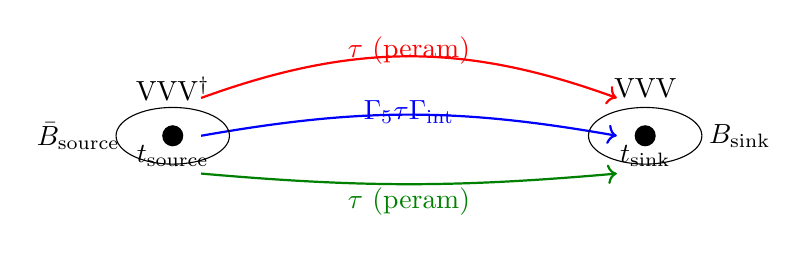
\begin{tikzpicture}[scale=1.2]
    % Source point
    \filldraw (0,0) circle (3pt) node[below] {$t_{\text{source}}$};
    \node at (0,0.5) {VVV$^\dagger$};
    % Sink point
    \filldraw (5,0) circle (3pt) node[below] {$t_{\text{sink}}$};
    \node at (5,0.5) {VVV};
    % Quark propagators
    \draw[->,red,thick] (0.3,0.4) to[bend left=20] (4.7,0.4);
    \draw[->,blue,thick] (0.3,0.0) to[bend left=10] (4.7,0.0);
    \draw[->,green!50!black,thick] (0.3,-0.4) to[bend right=5] (4.7,-0.4);
    % Labels
    \node[red] at (2.5,0.9) {$\tau$ (peram)};
    \node[blue] at (2.5,0.25) {$\Gamma_5\tau\Gamma_{\text{int}}$};
    \node[green!50!black] at (2.5,-0.7) {$\tau$ (peram)};
    % Source baryon
    \draw (0,0) ellipse (0.6 and 0.3);
    \node at (-1.0,0) {$\bar{B}_{\text{source}}$};
    % Sink baryon
    \draw (5,0) ellipse (0.6 and 0.3);
    \node at (6.0,0) {$B_{\text{sink}}$};
\end{tikzpicture}

图: 质子2pt关联函数的Wick收缩示意图：三个夸克传播子连接源和汇
\end{center}

两个contract项对应于两个Wick收缩（直接项和交换项）。
Dirac空间缩并的结果是一个$4\times 4$矩阵\texttt{[i,l]}：
\begin{equation}
    C_2(t_{\text{sink}}, t_{\text{source}})_{il} =
    \braket{ B_i(t_{\text{sink}}) \, \bar{B}_l(t_{\text{source}}) }
\end{equation}

其中$B_i$是插值算符（interpolator），通常取为：
\begin{equation}
    B_\alpha = \varepsilon_{abc} (u_a^T C\gamma_5 d_b) u_{c,\alpha}
\end{equation}
\end{physbox}

\subsection{宇称投影}

强子关联函数需要投影到确定的宇称态。在DeGrand-Rossi基下：

\begin{codebox}[宇称投影 (2pt script)]
\begin{lstlisting}[style=pythonstyle]
matrix_pplus  = 0.5 * (gamma(0) + gamma(4))   # 正宇称: (1+gamma4)/2
matrix_pminus = 0.5 * (gamma(0) - gamma(4))   # 负宇称: (1-gamma4)/2

# 投影到正/负宇称
contrac_nucl_pp = contract("li,yxil->yx", matrix_pplus,  contrac_nucl_matrix)
contrac_nucl_pm = contract("li,yxil->yx", matrix_pminus, contrac_nucl_matrix)

# 反周期边界条件的符号修正
for t_source in range(0, Nt):
    for t_sink in range(0, Nt):
        if t_sink < t_source:
            contrac_nucl_pp[t_sink, t_source] *= -1.0
        if t_sink > t_source:
            contrac_nucl_pm[t_sink, t_source] *= -1.0
\end{lstlisting}
\end{codebox}

\begin{physbox}[宇称投影算符]
在欧几里得空间中，正/负宇称投影算符为：
\begin{equation}
    \Gamma_{\pm} = \frac{1}{2}(1 \pm \gamma_4)
    \label{eq:parity_projector}
\end{equation}

在DeGrand-Rossi (DR) 手征基下，$\gamma_4$是非对角的：
\begin{equation}
    \gamma_4^{\text{DR}} = \begin{pmatrix}
        0 & 0 & 1 & 0 \\
        0 & 0 & 0 & 1 \\
        1 & 0 & 0 & 0 \\
        0 & 1 & 0 & 0
    \end{pmatrix}
\end{equation}

因此$\Gamma_+ = \frac{1}{2}(\mathbb{1} + \gamma_4)$筛选正宇称态，
$\Gamma_- = \frac{1}{2}(\mathbb{1} - \gamma_4)$筛选负宇称态。

\textbf{反周期边界条件}：费米子场在时间方向满足反周期边界条件
$\psi(t+N_t) = -\psi(t)$。当$t_{\text{sink}} < t_{\text{source}}$时（即关联函数"绕回"），
需要乘上$-1$因子来正确处理边界的相位。
\end{physbox}

% ============================================================================
% SECTION 6: Gamma矩阵
% ============================================================================
\section{Gamma矩阵：DeGrand-Rossi (DR) 基}

\subsection{DR基的显式表示}

donghx代码使用DeGrand-Rossi (DR) 手征基~\cite{DeGrand_Rossi}表示gamma矩阵。
DR基是手征表示的一种变体，其中$\gamma_5$是对角的：

\begin{physbox}[DR基Gamma矩阵]
\begin{align}
    \gamma_0^{\text{DR}} &= \mathbb{1}_{4\times4} &
    \gamma_1^{\text{DR}} &= \begin{pmatrix}
        0 & 0 & 0 & i \\
        0 & 0 & i & 0 \\
        0 & -i & 0 & 0 \\
        -i & 0 & 0 & 0
    \end{pmatrix} \\[0.3cm]
    \gamma_2^{\text{DR}} &= \begin{pmatrix}
        0 & 0 & 0 & -1 \\
        0 & 0 & 1 & 0 \\
        0 & 1 & 0 & 0 \\
        -1 & 0 & 0 & 0
    \end{pmatrix} &
    \gamma_3^{\text{DR}} &= \begin{pmatrix}
        0 & 0 & i & 0 \\
        0 & 0 & 0 & -i \\
        -i & 0 & 0 & 0 \\
        0 & i & 0 & 0
    \end{pmatrix} \\[0.3cm]
    \gamma_4^{\text{DR}} &= \begin{pmatrix}
        0 & 0 & 1 & 0 \\
        0 & 0 & 0 & 1 \\
        1 & 0 & 0 & 0 \\
        0 & 1 & 0 & 0
    \end{pmatrix} &
    \gamma_5^{\text{DR}} &= \begin{pmatrix}
        1 & 0 & 0 & 0 \\
        0 & 1 & 0 & 0 \\
        0 & 0 & -1 & 0 \\
        0 & 0 & 0 & -1
    \end{pmatrix}
\end{align}
\end{physbox}

\subsection{代码实现}

\begin{codebox}[Gamma矩阵定义 — gamma\_matrix\_cupy\_DR.py:6-109]
\begin{lstlisting}[style=pythonstyle]
import cupy as cp

g0 = cp.eye(4, dtype=complex)  # identity

g1 = cp.zeros((4,4), dtype=complex)
g1[0,3] = 1j; g1[1,2] = 1j; g1[2,1] = -1j; g1[3,0] = -1j

g2 = cp.zeros((4,4), dtype=complex)
g2[0,3] = -1; g2[1,2] = 1; g2[2,1] = 1; g2[3,0] = -1

g3 = cp.zeros((4,4), dtype=complex)
g3[0,2] = 1j; g3[1,3] = -1j; g3[2,0] = -1j; g3[3,1] = 1j

g4 = cp.zeros((4,4), dtype=complex)
g4[0,2] = 1; g4[1,3] = 1; g4[2,0] = 1; g4[3,1] = 1

g5 = cp.zeros((4,4), dtype=complex)
g5[0,0] = 1; g5[1,1] = 1; g5[2,2] = -1; g5[3,3] = -1
\end{lstlisting}
\end{codebox}

\subsection{插值算符 (Interpolator) 的构造}

插值算符是gamma矩阵的组合，用于构造具有特定量子数的强子算符：

\begin{codebox}[插值算符构造 — gamma\_matrix\_cupy\_DR.py:49-106]
\begin{lstlisting}[style=pythonstyle]
def gamma(i):
    if i == 0:  return g0                          # identity
    elif i == 1:  return g1                        # gamma1
    elif i == 2:  return g2                        # gamma2
    elif i == 3:  return g3                        # gamma3
    elif i == 4:  return g4                        # gamma4
    elif i == 5:  return g5                        # gamma5
    elif i == 6:  return cp.matmul(g2, g3)         # -gamma1*gamma4*gamma5
    elif i == 7:  return cp.matmul(g3, g1)         # -gamma2*gamma4*gamma5
    elif i == 8:  return cp.matmul(g1, g2)         # -gamma3*gamma4*gamma5
    elif i == 9:  return cp.matmul(g1, g4)         # gamma1*gamma4
    elif i == 10: return cp.matmul(g2, g4)         # gamma2*gamma4
    elif i == 11: return cp.matmul(g3, g4)         # gamma3*gamma4
    elif i == 12: return cp.matmul(g1, g5)         # gamma1*gamma5
    elif i == 13: return cp.matmul(g2, g5)         # gamma2*gamma5
    elif i == 14: return cp.matmul(g3, g5)         # gamma3*gamma5
    elif i == 15: return cp.matmul(g4, g5)         # gamma4*gamma5
    elif i == 16:                                   # (gamma3*gamma1)*(1+gamma4)/2
        return cp.matmul(cp.matmul(g3,g1), 0.5*(g0+g4))
    elif i == 17:                                   # (gamma3*gamma1)*(1-gamma4)/2
        return cp.matmul(cp.matmul(g3,g1), 0.5*(g0-g4))
\end{lstlisting}
\end{codebox}

\begin{physbox}[插值算符与质子量子数]
在2pt代码中，关键的插值算符组合包括（\texttt{element="\_Cg5g4"}时）：
\begin{equation}
    \Gamma_{\text{proj}} = \gamma_7 = -\gamma_2\gamma_4\gamma_5 = \gamma_3\gamma_1
    \label{eq:interpolator}
\end{equation}

这对应于$\gamma_3\gamma_1$型插值算符，用于筛选质子的特定自旋态。
插值算符的完整作用形式为：
\begin{equation}
    \tau \to \Gamma_{\text{proj}} \cdot \tau \cdot \Gamma_{\text{proj}}
\end{equation}

即对perambulator的Dirac指标同时从左右两侧进行投影。
\end{physbox}

% ============================================================================
% SECTION 7: GPU计算与数据管理
% ============================================================================
\section{GPU计算策略与数据管理}

\subsection{CuPy后端}

donghx代码主要使用CuPy作为GPU计算后端（\texttt{\_gpu.py}文件）。
CuPy提供了与NumPy兼容的API，但在GPU上执行：

\begin{codebox}[GPU数据传输 — 多处示例]
\begin{lstlisting}[style=pythonstyle]
import cupy as cp

# CPU -> GPU: 将numpy数组传到GPU
eigvecs_cupy = cp.asarray(Eigvec)
peram_cupy = cp.array(peram)

# GPU -> CPU: 将结果取回CPU
result_np = cp.asnumpy(gpu_result)

# GPU张量缩并
result = contract("abc,ade,bdf,cef->", A, B, C, D)

# GPU内存管理
cp._default_memory_pool.free_all_blocks()
cp.cuda.Device().synchronize()
\end{lstlisting}
\end{codebox}

\subsection{内存管理策略}

面对大规模格点数据，代码采用了多种内存管理策略：

\begin{enumerate}[label=(\arabic*), leftmargin=*]
    \item \textbf{按需读入:} perambulator按$t_{\text{source}}$逐个读入，而非一次性加载全部时间片。
    这大幅减少了GPU显存占用（典型情况：$N_t=64$时减少约64倍）。

    \item \textbf{空间分块 (Tiling):} VVV计算中将$x$方向分成$N_x$块，逐块缩并后累加。
    这避免了中间张量$\mathcal{O}(N_{\text{ev}}^3 \times N_x^3)$的巨大内存占用。

    \item \textbf{显式内存释放:} 使用\texttt{cp.\_default\_memory\_pool.free\_all\_blocks()}在每个$t_{\text{source}}$循环后释放GPU内存。

    \item \textbf{预计算与缓存:} Plaquette可以预先计算并存储为.npz文件（\texttt{Calc\_pla.py}），
    后续OPE算符计算直接加载（\texttt{Calc\_ope\_unpol\_new.py}），避免重复计算。
\end{enumerate}

\subsection{opt\_einsum加速}

代码中使用\texttt{opt\_einsum.contract}替代NumPy/CuPy原生的\texttt{einsum}，
利用优化的缩并路径减少计算量：

\begin{codebox}[opt\_einsum使用]
\begin{lstlisting}[style=pythonstyle]
from opt_einsum import contract

# 自动寻找最优缩并路径的einsum
result = contract("abc,gjad,gjbe,ilcf,def->il",
                  VVV_sink[t_sink], peram_u[t_sink],
                  CG5peram_uCG5[t_sink], peram_u[t_sink],
                  VVV_source)
\end{lstlisting}
\end{codebox}

对于复杂的多张量缩并（如质子2pt中的五张量缩并），
\texttt{opt\_einsum}通过动态规划找到计算量最小的缩并顺序，
通常能将计算复杂度降低一个量级。

\subsection{DCU（AMD/Hygon）后端}

以\texttt{\_dcu.py}结尾的文件使用DCU后端（AMD ROCm/HIP），
通过PyTorch兼容层实现GPU计算。
这些文件的代码结构与GPU版本相似，但使用PyTorch张量代替CuPy。

\subsection{文件I/O与数据格式}

\begin{table}[htbp]
\centering
\caption{donghx代码中的文件I/O格式汇总}
\label{tab:file_formats}
\begin{tabular}{@{}llll@{}}
\toprule
\textbf{数据类型} & \textbf{文件格式} & \textbf{读入方法} & \textbf{示例文件} \\
\midrule
规范组态 & ILDG二进制 & \texttt{np.fromfile} & \texttt{...ildg-binary-data} \\
本征矢量 & 原始二进制 (f8) & \texttt{np.fromfile} & \texttt{eigvecs\_t000\_20000} \\
Perambulator & 原始二进制 (f8) & \texttt{np.fromfile} & \texttt{perams.20000.0.0} \\
VVV & 原始二进制 (f8) & \texttt{np.fromfile} & \texttt{VVV.t000.Px0Py0Pz3.conf20000} \\
VdV & 原始二进制 (f8) & \texttt{np.fromfile} & \texttt{VdaggerV.Px0Py0Pz3.conf20000} \\
Plaquette & NumPy npz & \texttt{np.load} & \texttt{ops\_pla\_conf20000.npz} \\
OPE结果 & NumPy npy & \texttt{np.save/np.load} & \texttt{ops\_mu3\_nu0\_dz15\_conf20000.npy} \\
2pt结果 & NumPy npy & \texttt{cp.save/np.load} & \texttt{twopt\_slice\_pp\_Px3Py0Pz0\_...npy} \\
2pt结果(ASCII) & 文本dat & \texttt{write\_data\_ascii} & \texttt{corr\_Nucleon\_pp\_...dat} \\
\bottomrule
\end{tabular}
\end{table}

% ============================================================================
% SECTION 8: 完整计算流程
% ============================================================================
\section{完整计算流程与数据流}

\subsection{端到端流程}

图\ref{fig:workflow}展示了从规范组态到胶子PDF的完整计算数据流：

\begin{center}
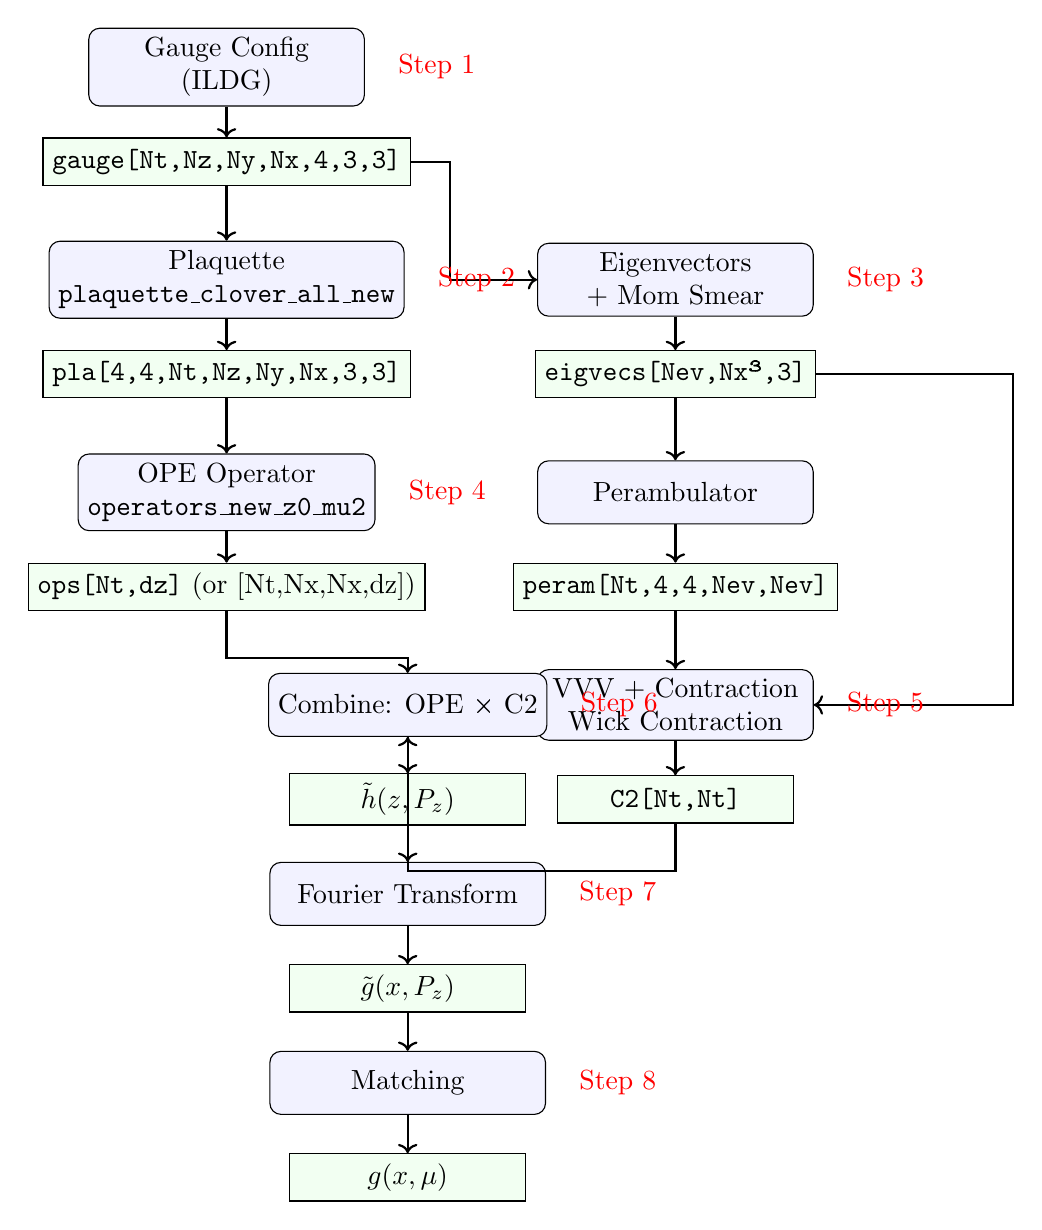
\begin{tikzpicture}[
    node distance=1.2cm,
    box/.style={rectangle,draw,rounded corners,minimum width=3.5cm,minimum height=0.8cm,align=center,fill=blue!5},
    data/.style={rectangle,draw,minimum width=3cm,minimum height=0.6cm,align=center,fill=green!5},
    arrow/.style={->,thick}
]
    % Nodes
    \node[box] (gauge) {Gauge Config \\ (ILDG)};
    \node[data,below of=gauge] (gauge_data) {\texttt{gauge[Nt,Nz,Ny,Nx,4,3,3]}};

    \node[box,below of=gauge_data,yshift=-0.3cm] (pla) {Plaquette \\ \texttt{plaquette\_clover\_all\_new}};
    \node[data,below of=pla] (pla_data) {\texttt{pla[4,4,Nt,Nz,Ny,Nx,3,3]}};

    \node[box,right of=pla,xshift=4.5cm] (eig) {Eigenvectors \\ + Mom Smear};
    \node[data,below of=eig] (eig_data) {\texttt{eigvecs[Nev,Nx³,3]}};

    \node[box,below of=eig_data,yshift=-0.3cm] (peram) {Perambulator};
    \node[data,below of=peram] (peram_data) {\texttt{peram[Nt,4,4,Nev,Nev]}};

    \node[box,below of=pla_data,yshift=-0.3cm] (ope) {OPE Operator \\ \texttt{operators\_new\_z0\_mu2}};
    \node[data,below of=ope] (ope_data) {\texttt{ops[Nt,dz]} (or [Nt,Nx,Nx,dz])};

    \node[box,below of=peram_data,yshift=-0.3cm] (vvv) {VVV + Contraction \\ Wick Contraction};
    \node[data,below of=vvv] (c2_data) {\texttt{C2[Nt,Nt]}};

    \node[box,below of=ope_data,yshift=-0.3cm,xshift=2.3cm] (combine) {Combine: OPE × C2};
    \node[data,below of=combine] (h_data) {$\tilde{h}(z,P_z)$};

    \node[box,below of=h_data] (ft) {Fourier Transform};
    \node[data,below of=ft] (g_data) {$\tilde{g}(x,P_z)$};

    \node[box,below of=g_data] (match) {Matching};
    \node[data,below of=match] (pdf_data) {$g(x,\mu)$};

    % Arrows
    \draw[arrow] (gauge) -- (gauge_data);
    \draw[arrow] (gauge_data) -- (pla);
    \draw[arrow] (pla) -- (pla_data);
    \draw[arrow] (pla_data) -- (ope);
    \draw[arrow] (ope) -- (ope_data);

    \draw[arrow] (gauge_data.east) -- ++(0.5,0) |- (eig);
    \draw[arrow] (eig) -- (eig_data);
    \draw[arrow] (eig_data) -- (peram);
    \draw[arrow] (peram) -- (peram_data);
    \draw[arrow] (peram_data) -- (vvv);
    \draw[arrow] (eig_data.east) -- ++(2.5,0) |- (vvv);
    \draw[arrow] (vvv) -- (c2_data);

    \draw[arrow] (ope_data.south) -- ++(0,-0.6) -| (combine);
    \draw[arrow] (c2_data.south) -- ++(0,-0.6) -| (combine);
    \draw[arrow] (combine) -- (h_data);
    \draw[arrow] (h_data) -- (ft);
    \draw[arrow] (ft) -- (g_data);
    \draw[arrow] (g_data) -- (match);
    \draw[arrow] (match) -- (pdf_data);

    % Labels
    \node[right=0.3cm of gauge,text=red] {Step 1};
    \node[right=0.3cm of pla,text=red] {Step 2};
    \node[right=0.3cm of eig,text=red] {Step 3};
    \node[right=0.3cm of ope,text=red] {Step 4};
    \node[right=0.3cm of vvv,text=red] {Step 5};
    \node[right=0.3cm of combine,text=red] {Step 6};
    \node[right=0.3cm of ft,text=red] {Step 7};
    \node[right=0.3cm of match,text=red] {Step 8};
\end{tikzpicture}

图: 胶子PDF计算的完整数据流图：8个步骤从规范组态到光锥PDF
\end{center}

\subsection{各步骤的代码对应}

\begin{table}[htbp]
\centering
\caption{计算步骤与代码文件对应表}
\label{tab:step_code}
\begin{tabular}{@{}cll@{}}
\toprule
\textbf{步骤} & \textbf{物理内容} & \textbf{主要代码文件} \\
\midrule
1 & 规范场读入 & \texttt{Calc\_pla.py}, \texttt{Calc\_ope\_unpol.py} \\
2 & Plaquette/$F_{\mu\nu}$构造 & \texttt{Operator.py} (plaquette\_clover\_*) \\
3 & 本征矢量+动量涂抹 & \texttt{2pt\_proton\_Cg5gmu\_*\_gpu.py} \\
4 & OPE非定域算符 & \texttt{Calc\_ope\_unpol.py}, \texttt{Calc\_ope\_helicity.py} \\
5 & VVV+Wick收缩 & \texttt{Calc\_VVV.py}, \texttt{2pt\_proton\_Cg5gmu\_*\_gpu.py} \\
6 & 组合: OPE × C2 & zhangxin工作流 (\texttt{gluon\_pdf\_workflow.py}) \\
7 & Fourier变换 & zhangxin分析代码 (\texttt{main.py}) \\
8 & 微扰匹配 & LaMET匹配核代码 \\
\bottomrule
\end{tabular}
\end{table}

\subsection{典型运行命令}

\begin{codebox}[典型运行示例]
Plquette预计算：
\begin{lstlisting}[style=bashstyle]
python Calc_pla.py < pla_params.txt
# pla_params.txt:
#   Nt 64 / Nx 32 / conf_id 20000
#   conf_file /path/to/config.dat
#   pla_dir /path/to/output/
\end{lstlisting}

OPE算符计算（3-rank MPI）：
\begin{lstlisting}[style=bashstyle]
mpirun -np 3 python Calc_ope_unpol.py < ope_params.txt
# ope_params.txt:
#   Nt 64 / Nx 32 / delta_z 15 / conf_id 20000
#   conf_file /path/to/config.dat
#   link_dir z
#   output_dir /path/to/ope_output/
\end{lstlisting}

质子2pt关联函数（GPU单卡）：
\begin{lstlisting}[style=bashstyle]
python 2pt_proton_Cg5gmu_L32x64_mom2_xdir_gpu.py 20000
# 硬编码参数: Nt=64, Nx=32, Nev=100, Pz=0, mom_smear=3
# 关键输出: twopt_slice_pp_Px3Py0Pz0_...npy
\end{lstlisting}
\end{codebox}

% ============================================================================
% SECTION 9: 总结
% ============================================================================
\section{总结}

本文档系统地分析了 donghx 在 \texttt{/root/lattice-pdf/examples/donghx/} 中的全部格点QCD代码，
建立了物理公式与GPU代码实现之间的一一对应关系。主要涵盖以下内容：

\begin{enumerate}[leftmargin=*]
    \item \textbf{理论框架}: LaMET方法将格点上的准PDF与光锥PDF通过微扰匹配联系起来。
    胶子PDF涉及非连通图，三点关联函数被分解为质子2pt部分和OPE胶子算符部分。

    \item \textbf{场强张量构造}: 格点上的$F_{\mu\nu}$通过Clover（四叶草）改进的plaquette构造，
    四个定向plaquette的对称组合将离散化误差降至$\mathcal{O}(a^2)$。
    代码中通过\texttt{plaquette\_clover\_all\_new}和\texttt{plaquette\_clover\_all\_tilde}
    分别计算$F_{\mu\nu}$和其对偶$\tilde{F}_{\mu\nu}$。

    \item \textbf{非定域OPE算符}: 通过Wilson线连接两个位置的场强张量。
    \texttt{operators\_new\_z0\_mu2}等函数实现了各种空间构型（正向/反向Wilson线、
    不同Lorentz指标组合）。
    MPI并行将不同$(\mu,\nu)$分量分配给不同进程。

    \item \textbf{质子2pt关联函数}: 使用distillation方法，通过低模拉普拉斯本征矢量、
    perambulator和VVV三重量子数进行Wick收缩。
    动量涂抹通过注入平面波相位$\exp(-i\vec{\zeta}\cdot\vec{x})$提高高动量态overlap。

    \item \textbf{GPU优化}: CuPy后端、opt\_einsum缩并优化、按需读入、
    空间分块和显式内存管理等策略保证了在大规模格点上的计算效率。
\end{enumerate}

本分析覆盖了donghx目录中的68个文件，包括核心模块(\texttt{Operator.py},
\texttt{gamma\_matrix\_cupy\_DR.py}, \texttt{input\_output\_4\_cupy.py})、
OPE计算脚本(\texttt{Calc\_ope\_unpol.py}, \texttt{Calc\_ope\_helicity.py},
\texttt{Calc\_ope\_gauge\_fix\_unpol.py}, \texttt{Calc\_ope\_helicity\_new.py},
\texttt{Calc\_ope\_unpol\_new.py}, \texttt{Calc\_ope\_helicity\_test.py},
\texttt{Calc\_ope\_gauge\_fix\_helicity.py})、
plaquette预计算(\texttt{Calc\_pla.py})、
VVV计算(\texttt{Calc\_VVV.py})、
质子2pt脚本（40+个变体，覆盖不同格点尺寸、动量和GPU/DCU后端）以及
数据检查工具(\texttt{check\_exist.py}, \texttt{check\_exist\_TMD.py})。

% ============================================================================
% 参考文献
% ============================================================================
\begin{thebibliography}{99}

\bibitem{Ji:2013dva}
X.~Ji,
``Parton Physics on a Euclidean Lattice,''
Phys.\ Rev.\ Lett.\ \textbf{110}, 262002 (2013)
[\href{https://arxiv.org/abs/1305.1539}{arXiv:1305.1539}].

\bibitem{Ji:2014gla}
X.~Ji,
``Parton Physics from Large-Momentum Effective Field Theory,''
Sci.\ China Phys.\ Mech.\ Astron.\ \textbf{57}, 1407-1412 (2014)
[\href{https://arxiv.org/abs/1404.6680}{arXiv:1404.6680}].

\bibitem{Ji:2020ect}
X.~Ji, Y.-S.~Liu, Y.~Liu, J.-H.~Zhang, and Y.~Zhao,
``Large-Momentum Effective Theory,''
Rev.\ Mod.\ Phys.\ \textbf{93}, no.3, 035005 (2021)
[\href{https://arxiv.org/abs/2004.03543}{arXiv:2004.03543}].

\bibitem{Note_of_gluon_PDFs}
内部理论笔记,
``Note of gluon PDFs,''
\texttt{/root/lattice-pdf/docs/Note of gluon PDFs.pdf}.

\bibitem{First_Nucleon_Gluon_PDF}
T.~Khan \textit{et al.} (HadStruc Collaboration),
``First Nucleon Gluon PDF from Large Momentum Effective Theory,''
[\href{https://arxiv.org/abs/XXXX.XXXXX}{arXiv preprint}].
(见 \texttt{/root/lattice-pdf/docs/First Nucleon Gluon PDF from Large Momentum Effective Theory.pdf})

\bibitem{Gluon_Quasi_PDF}
W.~Wang, J.-H.~Zhang, S.~Zhao, and R.~Zhu,
``Gluon Quasi-PDF From Lattice QCD,''
Phys.\ Rev.\ D \textbf{100}, 074509 (2019).
(见 \texttt{/root/lattice-pdf/docs/Gluon Quasi-PDF From Lattice QCD.pdf})

\bibitem{Distillation_High_Momentum}
C.~Egerer \textit{et al.} (HadStruc Collaboration),
``Distillation at High-Momentum,''
Phys.\ Rev.\ D \textbf{103}, 034502 (2021)
[\href{https://arxiv.org/abs/2009.10891}{arXiv:2009.10891}].
(见 \texttt{/root/lattice-pdf/docs/Distillation at High-Momentum.pdf})

\bibitem{Peardon_2009}
M.~Peardon \textit{et al.} (Hadron Spectrum Collaboration),
``A Novel Quark-Field Creation Operator Construction for Hadronic Physics in Lattice QCD,''
Phys.\ Rev.\ D \textbf{80}, 054506 (2009)
[\href{https://arxiv.org/abs/0905.2160}{arXiv:0905.2160}].

\bibitem{Kinematically_enhanced}
G.~Bali, B.~Lang, B.~Lucini, B.~L\"uscher, and S.~Romiti,
``Kinematically-Enhanced Interpolating Operators for Boosted Hadrons,''
(见 \texttt{/root/lattice-pdf/docs/Kinematically-enhanced interpolating operators for boosted hadrons.pdf})

\bibitem{Bali_2016}
G.~Bali \textit{et al.},
``Momentum-Smeared Interpolating Operators,''
(2016).

\bibitem{DeGrand_Rossi}
T.~DeGrand and P.~Rossi,
``Conditioning Techniques for Dynamical Fermions,''
Comput.\ Phys.\ Commun.\ \textbf{60}, 211 (1990).

\bibitem{Gattringer_Lang}
C.~Gattringer and C.~B.~Lang,
\textit{Quantum Chromodynamics on the Lattice},
Springer (2010).
(见 \texttt{/root/lattice-pdf/books/Quantum Chromodynamics on the Lattice.pdf})

\bibitem{Hybrid_Renorm}
X.~Ji, Y.~Liu, A.~Sch\"afer, W.~Wang, Y.-B.~Yang, J.-H.~Zhang, and Y.~Zhao,
``A Hybrid Renormalization Scheme for Quasi Light-Front Correlations in Large-Momentum Effective Theory,''
Nucl.\ Phys.\ B \textbf{964}, 115311 (2021).
(见 \texttt{/root/lattice-pdf/docs/A Hybrid Renormalization Scheme for Quasi Light-Front Correlations in Large-Momentum Effective Theory.pdf})

\bibitem{Self_Renorm_Gluon}
``First Self-Renormalized Gluon PDF of Nucleon from Large-Momentum Effective Theory in the Continuum Limit,''
(见 \texttt{/root/lattice-pdf/docs/First Self-Renormalized Gluon PDF of Nucleon from Large-Momentum Effective Theory in the Continuum Limit.pdf})

\bibitem{Gauge_Fixing}
Y.~Li \textit{et al.},
``Impact of gauge fixing precision on the continuum limit of non-local quark-bilinear lattice operators,''
(见 \texttt{/root/lattice-pdf/docs/Impact of gauge fixing precision on the continuum limit of non-local quark-bilinear lattice operators.pdf})

\bibitem{leading_power}
``Leading Power Accuracy in Lattice Calculations of Parton Distributions,''
(见 \texttt{/root/lattice-pdf/docs/Leading Power Accuracy in Lattice Calculations of Parton Distributions.pdf})

\bibitem{clover_improvement}
B.~Sheikholeslami and R.~Wohlert,
``Improved Continuum Limit Lattice Action for QCD with Wilson Fermions,''
Nucl.\ Phys.\ B \textbf{259}, 572 (1985).

\bibitem{Luscher_2010}
M.~L\"uscher,
``Properties and uses of the Wilson flow in lattice QCD,''
JHEP \textbf{08}, 071 (2010)
[\href{https://arxiv.org/abs/1006.4518}{arXiv:1006.4518}].

\bibitem{Continuum_Gluon_PDF}
``Gluon Parton Distribution of the Nucleon from 2+1+1-Flavor Lattice QCD in the Physical-Continuum Limit,''
(见 \texttt{/root/lattice-pdf/docs/Gluon Parton Distribution of the Nucleon from 2+1+1-Flavor Lattice QCD in the Physical-Continuum Limit.pdf})

\end{thebibliography}

\end{document}
